\documentclass[
  size=12pt,
  paper=screen,
  mode=present,
%%  display=slidenotes,
  %style=tycja
  style=sailor
]{powerdot}
%% Presentation Setup (footers, transitions, slide numbering)
\pdsetup{
  lf=ENEE631: Digital Image Processing,
  rf=Naotoshi Seo David~A. Schug,
  trans=Wipe,
  theslide=\arabic{slide}
}
\usepackage{graphics,graphicx,latexsym,amssymb,amsmath,amsfonts,natbib,bibentry,subfigure}
%% Title slide
  \title{Image Matching Using Scale Invariant Feature Transform (SIFT)\\}
  		
  \author{Naotoshi Seo\\David~A. Schug\\}
  \date{May 18, 2007}

%% begin document
\begin{document}
  \maketitle %% make the title slide

%% Create table of contents slide
%\begin{slide}[toc=,bm=]{Table of Contents}
%  \tableofcontents[content=sections]
%\end{slide}

%% Begin section on Trigonometric Series
\section[tocsection=true,slide=false]{Overview}

\begin{slide}{Image Matching}
  \begin{figure}
    \begin{center}
      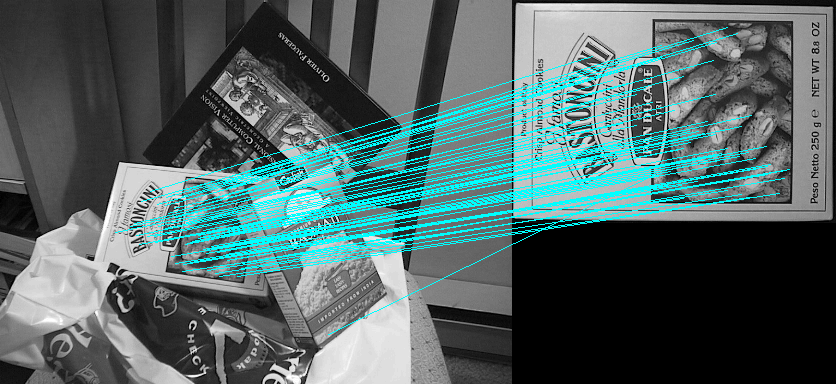
\includegraphics[width=10cm]{../../images/BookSceneMatchLowe.eps}
    \end{center}
  \end{figure}
\end{slide}

\begin{slide}{Interest point detector}
  \begin{figure}
    \begin{center}
      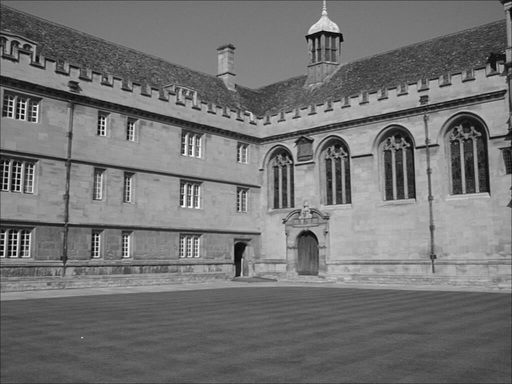
\includegraphics[width=9cm]{../../images/wadham001.eps}
    \end{center}
  \end{figure}
\end{slide}

\begin{slide}{Harris corner detector}
  \begin{figure}
    \begin{center}
      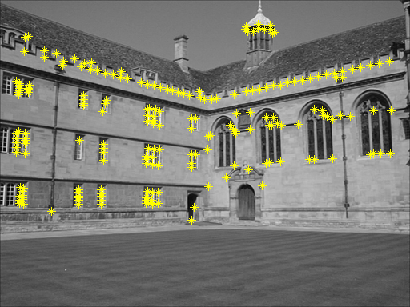
\includegraphics[width=9cm]{../../images/Harriswadham001.eps}
    \end{center}
  \end{figure}
\end{slide}

\begin{slide}{Defect of corner detector}
  Non-invariant to image scale
  \begin{figure}
    \begin{center}
      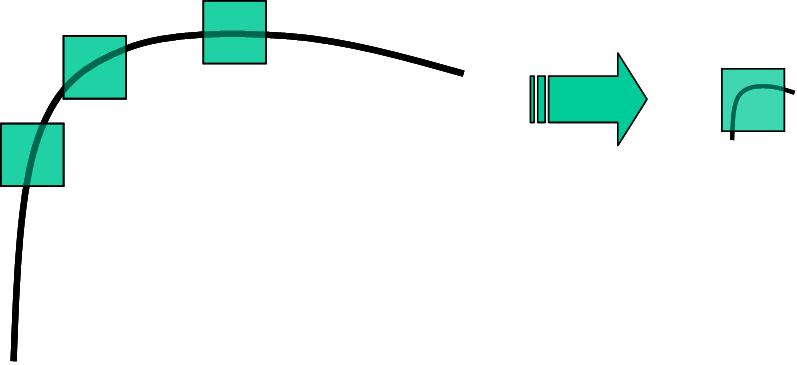
\includegraphics[width=7cm]{../HarrisScaleVariant.eps}
    \end{center}
  \end{figure}
  \begin{center}
  Edges~~~~~~~~~~~~ into ~~~~~~~~~~~~~~~~ Corner!
  \end{center}
\end{slide}

%% Begin section on Scale invariant feature transform
\section[tocsection=true,slide=false]{Scale Invariant Feature Transform}

\begin{slide}{SIFT Overview}
proposed by Lowe \bibentry{dLowe04} in 2004. 
\begin{enumerate}
\item \textbf{Scale-space construction} - construction of Gaussian and difference-of-Gaussian pyramids. 
\item \textbf{Keypoint localization} - keypoint candidates are chosen from the extrema in the scale space. 
\item \textbf{Orientation assignment} - orientations are assigned to each keypoint based on histograms of gradient directions computed in a 16x16 window. 
\item \textbf{Keypoint descriptor} - representation in a 128-dimensional vector.
\end{enumerate}

\noindent\textbf{Keypoint matching} - the best candidate match is found by its nearest neighbor.
\end{slide}

\begin{slide}{Scale Space Construction}
  Gaussian Pyramid
  \begin{figure}
    \begin{center}
      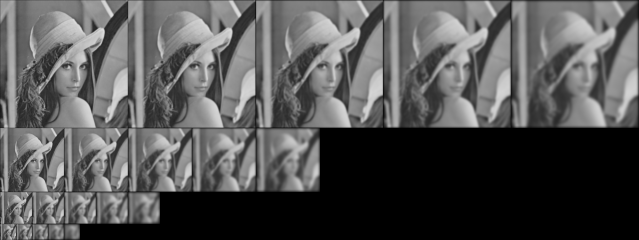
\includegraphics[width=10cm]{../../images/LenaGaussianPyramid.eps}
    \end{center}
  \end{figure}
\end{slide}

\begin{slide}{Scale Space Construction (Cont.)}
  Difference-of-Gaussian (DoG) Pyramid
  \begin{figure}
    \begin{center}
      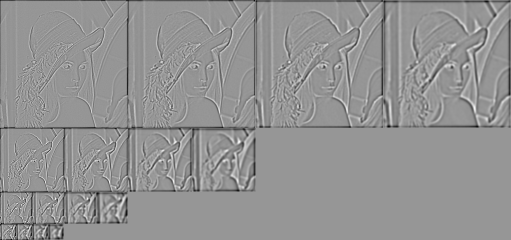
\includegraphics[width=10cm]{../../images/LenaDoGPyramid.eps}
    \end{center}
  \end{figure}
\end{slide}

\begin{slide}{Keypoint Localization}
  Find exterema in DoG Pyramids
  \begin{figure}
    \begin{center}
      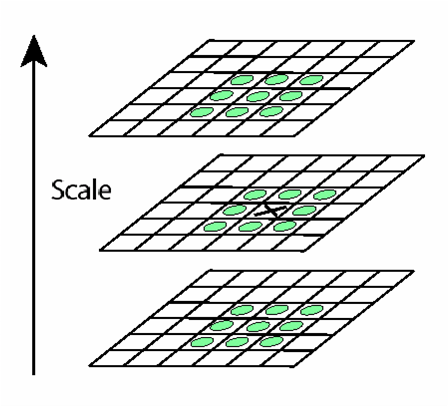
\includegraphics[width=5cm]{../Extrema.eps}
    \end{center}\label{Fi:EXT}
  \end{figure}
\end{slide}

\begin{slide}{Keypoint Localization (Cont.)}
  Result
  \begin{figure}
    \begin{center}
      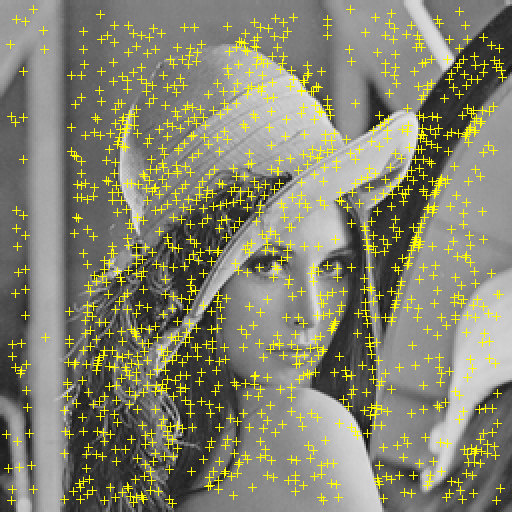
\includegraphics[width=5cm]{../../images/LenaKeypointExtrema.eps}\\
    \end{center}\label{Fi:EXT}
  \end{figure}
\end{slide}

\begin{slide}{Keypoint Localization (Cont.)}
  After removing low contrast points
  \begin{figure}
    \begin{center}
      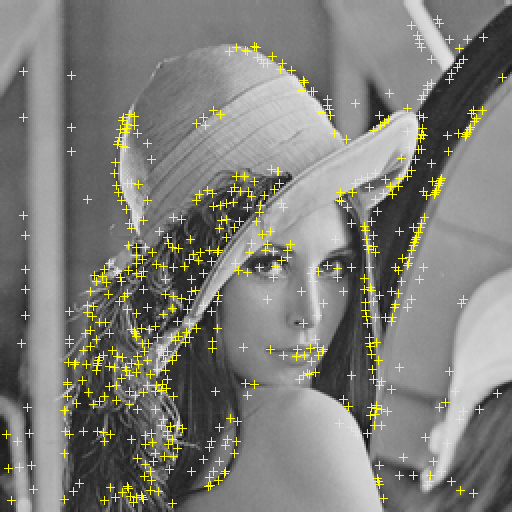
\includegraphics[width=5cm]{../../images/LenaKeypointRemoveLowContrast.eps}\\
    \end{center}\label{Fi:EXT}
  \end{figure}
\end{slide}

\begin{slide}{Keypoint Localization (Cont.)}
  After removing edge responses
  \begin{figure}
    \begin{center}
      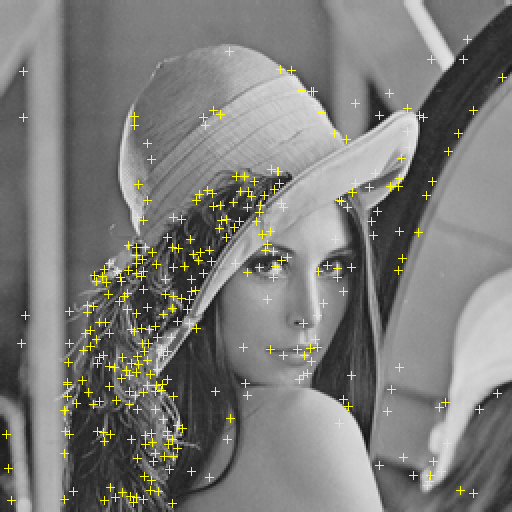
\includegraphics[width=5cm]{../../images/LenaKeypointRemoveEdge.eps}\\
    \end{center}\label{Fi:EXT}
  \end{figure}
\end{slide}

\begin{slide}{Orientation Assignment}
  \begin{figure}
    \begin{center}
      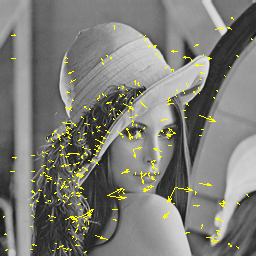
\includegraphics[width=7cm]{../../images/LenaOrientation.eps}\\
    \end{center}\label{Fi:EXT}
  \end{figure}
\end{slide}

\begin{slide}{Keypoint Descriptor}
  \begin{figure}
    \begin{center}
      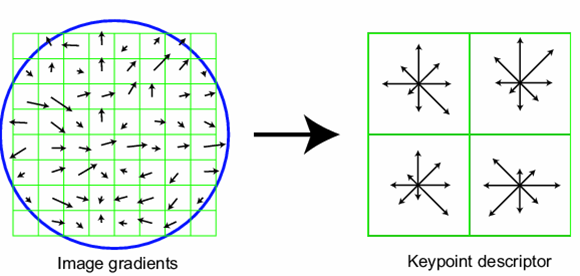
\includegraphics[width=8cm]{../KeypointDescriptor.eps}\\
    \end{center}\label{Fi:EXT}
  \end{figure}
\end{slide}

\begin{slide}{Image Matching}
  \begin{figure}
    \begin{center}
      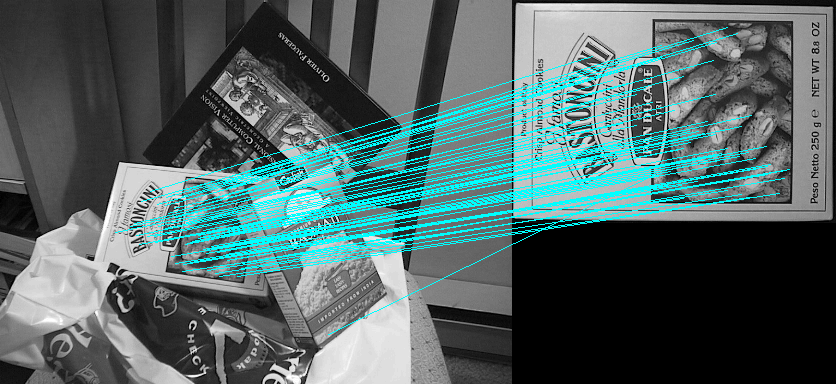
\includegraphics[width=10cm]{../../images/BookSceneMatchLowe.eps}
    \end{center}\label{Fi:EXT}
  \end{figure}
\end{slide}

\section[tocsection=true,slide=false]{Comparison with Harris}

\begin{slide}{Comparison with Harris}
  Interest point detector
  \begin{figure}
    \begin{center}
    \begin{tabular}{@{} cc @{}}
      \begin{minipage}{0.5\hsize}
        \begin{center}
          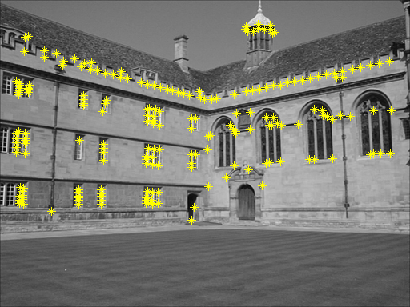
\includegraphics[width=4cm]{../../images/Harriswadham001.eps}\\
        \end{center}
      \end{minipage}    &
      \begin{minipage}{0.5\hsize}
        \begin{center}
          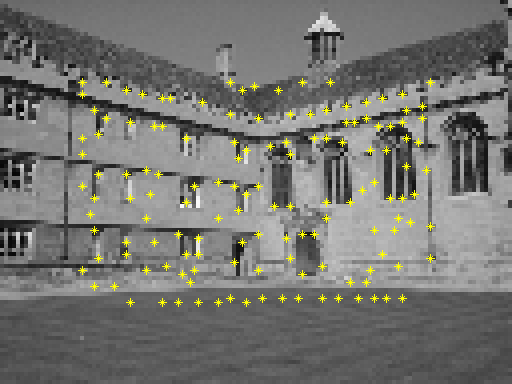
\includegraphics[width=4cm]{../../images/Harriswadham001S.eps}
        \end{center}
      \end{minipage}    \\
      \begin{minipage}{0.5\hsize}
        \begin{center}
          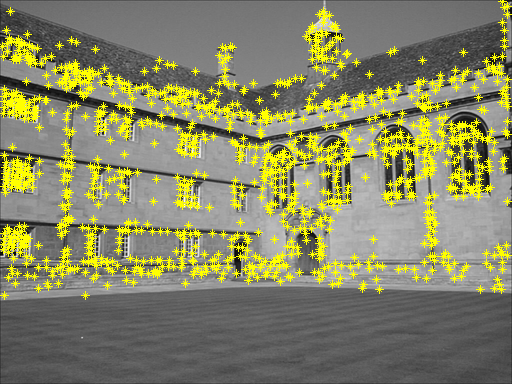
\includegraphics[width=4cm]{../../images/SIFTwadham001.eps}
        \end{center}
      \end{minipage}    &
      \begin{minipage}{0.5\hsize}
        \begin{center}
          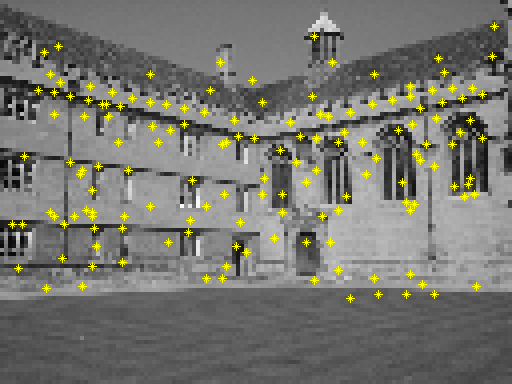
\includegraphics[width=4cm]{../../images/SIFTwadham001S.eps}
        \end{center}
      \end{minipage}    \\
    \end{tabular}
    \label{Fi:hoteltracks}
  \end{center}
  \end{figure}
\end{slide}

\begin{slide}{Comparison with Harris (Cont.)}
  Image matching
  \begin{figure}
  \begin{center}
    \begin{tabular}{@{} cc @{}}
      \begin{minipage}{0.6\hsize}
        \begin{center}
          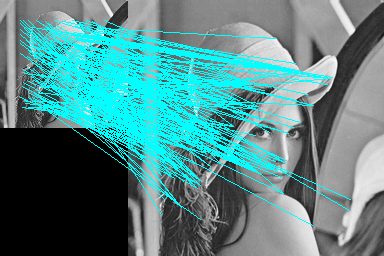
\includegraphics[width=5.5cm]{../../images/HarrisScaleInvariantTest05.eps}
        \end{center}
      \end{minipage}    &
      \begin{minipage}{0.4\hsize}
        \begin{center}
          Harris
        \end{center}
      \end{minipage}    \\
      \begin{minipage}{0.6\hsize}
        \begin{center}
          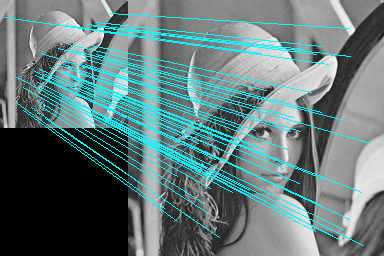
\includegraphics[width=5.5cm]{../../images/SIFTScaleInvariantTest05.eps}
        \end{center}
      \end{minipage}    &
      \begin{minipage}{0.4\hsize}
        \begin{center}
          SIFT
        \end{center}
      \end{minipage}    \\
    \end{tabular}
    \label{Fi:hoteltracks}
  \end{center}
\end{figure}

\end{slide}

\section[tocsection=true,slide=false]{Tracking}

\begin{slide}{Extension into Tracking}
Input Images
\begin{figure}
  \begin{center}
    \begin{tabular}{@{} ccc @{}}

      \begin{minipage}{0.33\hsize}
        \begin{center}
          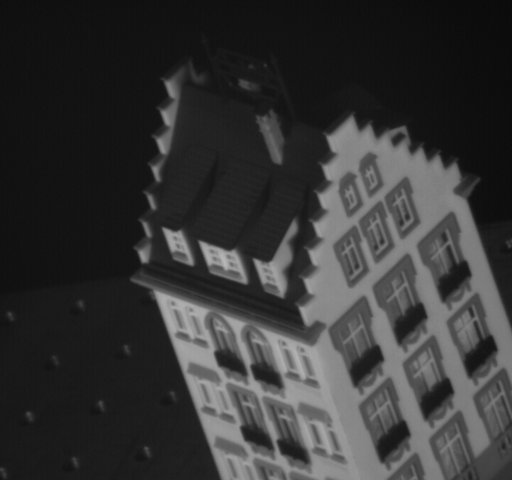
\includegraphics[width=3cm]{../../images/hotel/hotel1.eps}\\
          The 1st frame
        \end{center}
      \end{minipage}    &
      \begin{minipage}{0.33\hsize}
        \begin{center}
          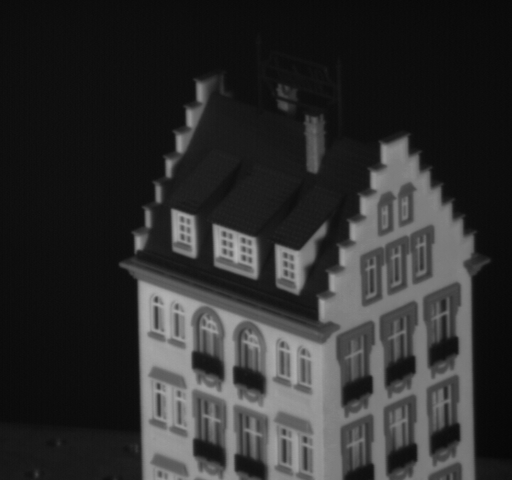
\includegraphics[width=3cm]{../../images/hotel/hotel50.eps}\\
          50th
        \end{center}
      \end{minipage}    
      \begin{minipage}{0.33\hsize}
        \begin{center}
          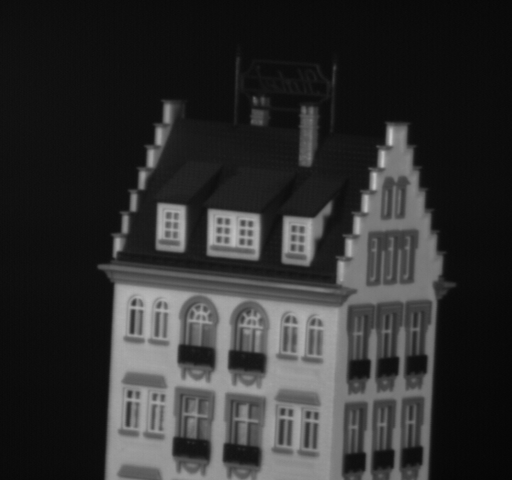
\includegraphics[width=3cm]{../../images/hotel/hotel100.eps}\\
          100th
        \end{center}
      \end{minipage}    
    \end{tabular}
    \label{fig:BaseLine}
  \end{center}
\end{figure} 

\end{slide}

\begin{slide}{Result}
\begin{figure}
  \begin{center}
    \begin{tabular}{@{} cc @{}}

      \begin{minipage}{0.5\hsize}
        \begin{center}
          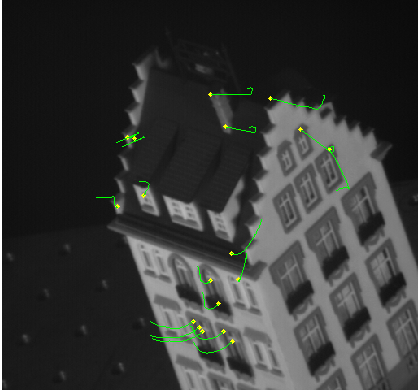
\includegraphics[width=4.5cm]{../../images/hotel/hoteltracked100.eps}\\
          SIFT
        \end{center}
      \end{minipage}    &
      \begin{minipage}{0.5\hsize}
        \begin{center}
          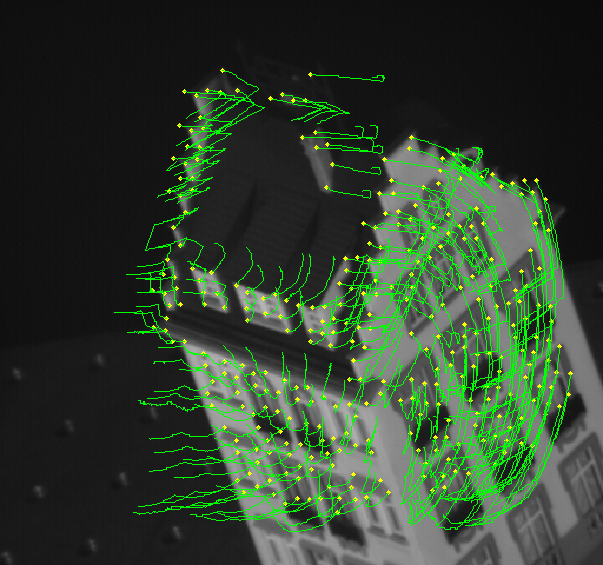
\includegraphics[width=4.5cm]{../../images/hotel/klttrack.eps}\\
          KLT
        \end{center}
      \end{minipage}    
    \end{tabular}
    \label{Fi:hoteltracks}
  \end{center}
\end{figure}
\end{slide}

\begin{slide}{The 2nd Experiment}
Input Images
\begin{figure}
  \begin{center}
    \begin{tabular}{@{} ccc @{}}

      \begin{minipage}{0.33\hsize}
        \begin{center}
          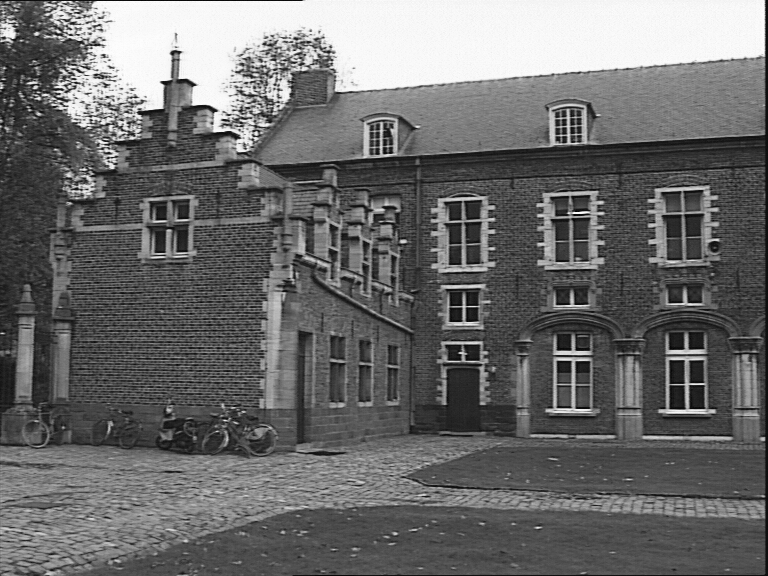
\includegraphics[width=3cm]{../../images/castle/castle001.eps}\\
          The 1st frame
        \end{center}
      \end{minipage}    &
      \begin{minipage}{0.33\hsize}
        \begin{center}
          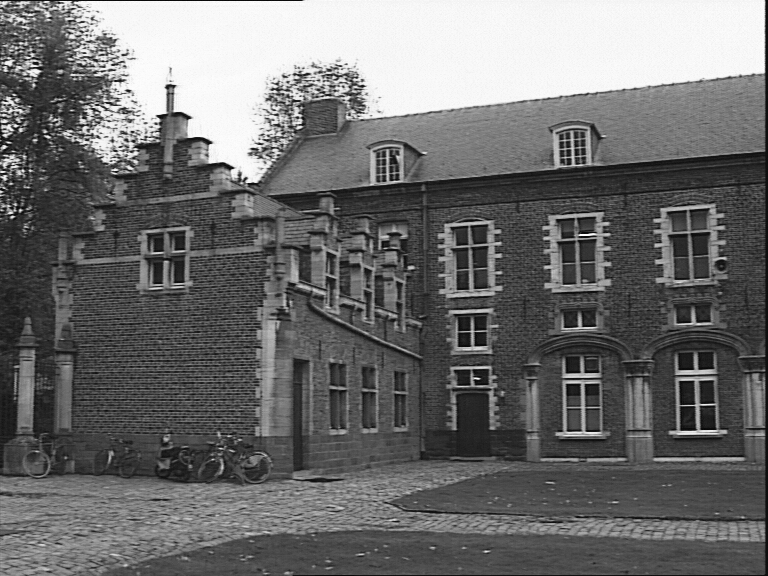
\includegraphics[width=3cm]{../../images/castle/castle002.eps}\\
          2nd
        \end{center}
      \end{minipage}    
      \begin{minipage}{0.33\hsize}
        \begin{center}
          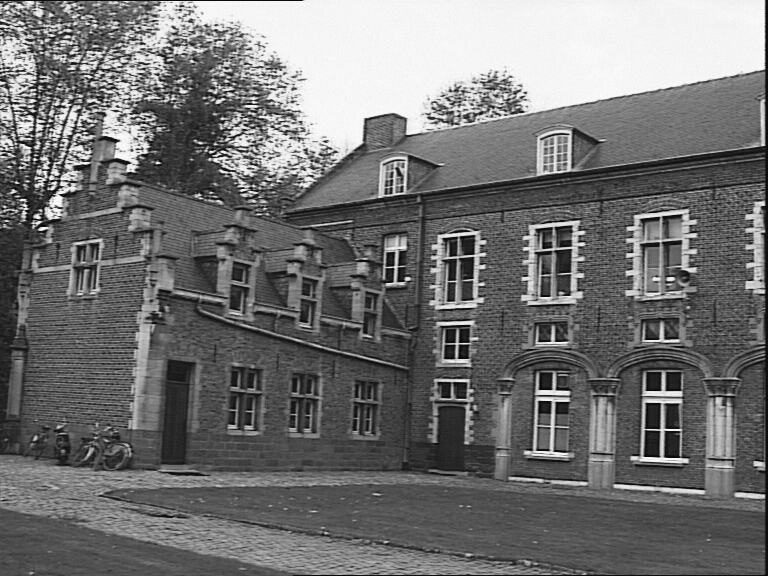
\includegraphics[width=3cm]{../../images/castle/castle013.eps}\\
          13th
        \end{center}
      \end{minipage}    
    \end{tabular}
    \label{fig:BaseLine}
  \end{center}
\end{figure} 

\end{slide}

\begin{slide}{Result and comparison with KLT Feature Tracking}
\begin{figure}
  \begin{center}
    \begin{tabular}{@{} cc @{}}

      \begin{minipage}{0.5\hsize}
        \begin{center}
          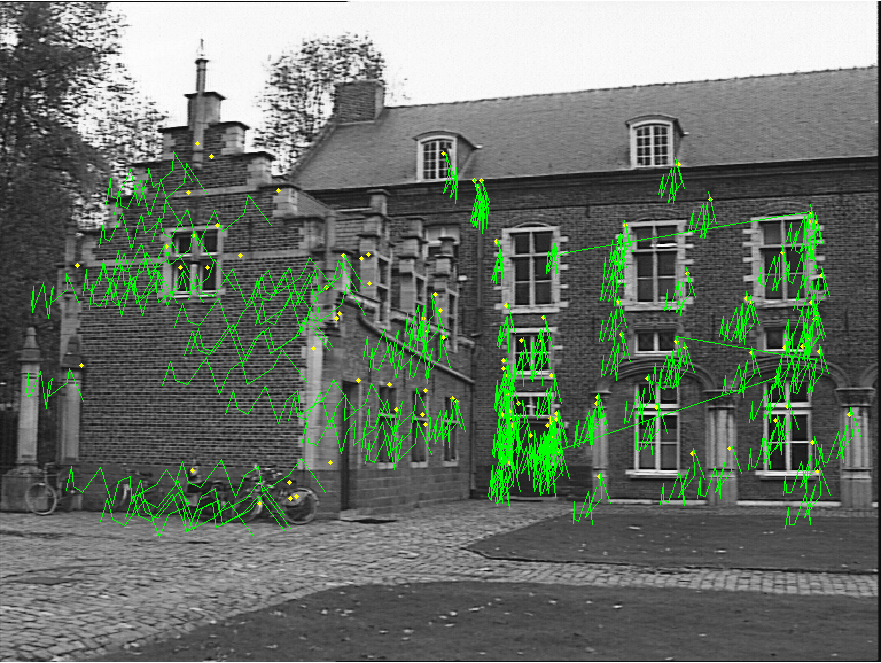
\includegraphics[width=4.5cm]{../../images/castle/SIFTcastle.eps}\\
          SIFT
        \end{center}
      \end{minipage}    &
      \begin{minipage}{0.5\hsize}
        \begin{center}
          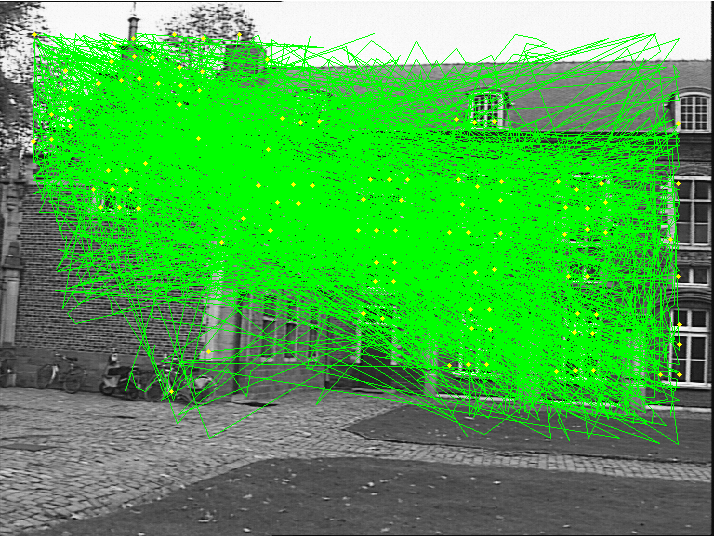
\includegraphics[width=4.5cm]{../../images/castle/KLTcastle.eps}\\
          KLT
        \end{center}
      \end{minipage}    
    \end{tabular}
    \label{Fi:hoteltracks}
  \end{center}
\end{figure}
\end{slide}

\section[tocsection=true,slide=false]{Another application}

\begin{slide}{Another example of interesting application}
Panoramic Image Stiching
\begin{figure}
  \begin{center}
    \begin{tabular}{@{} cc @{}}

      \begin{minipage}{0.5\hsize}
        \begin{center}
          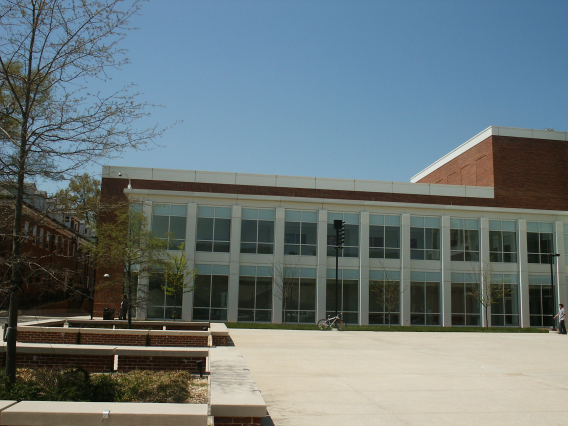
\includegraphics[width=4cm]{../../images/KIM/KIM3.eps}\\
        \end{center}
      \end{minipage}    &
      \begin{minipage}{0.55\hsize}
        \begin{center}
          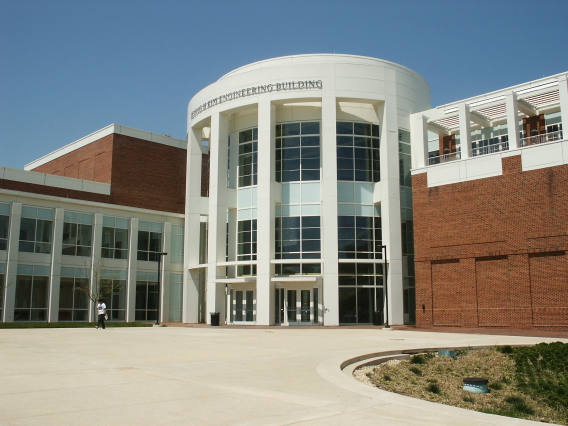
\includegraphics[width=4cm]{../../images/KIM/KIM2.eps}\\
        \end{center}
      \end{minipage}    \\
      \begin{minipage}{0.5\hsize}
        \begin{center}
          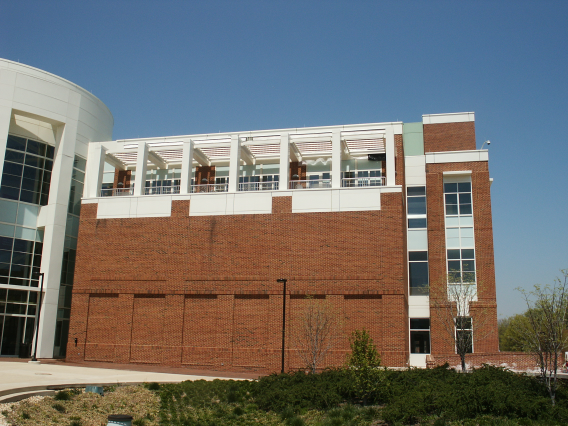
\includegraphics[width=4cm]{../../images/KIM/KIM1.eps}\\
        \end{center}
      \end{minipage}    &
      ~
      \\
    \end{tabular}
    \label{Fi:hoteltracks}
  \end{center}
\end{figure}
\end{slide}

\begin{slide}{Another example of interesting application}
Panorama Result
\begin{figure}
  \begin{center}
    \begin{tabular}{@{} c @{}}
      \begin{minipage}{1.0\hsize}
        \begin{center}
          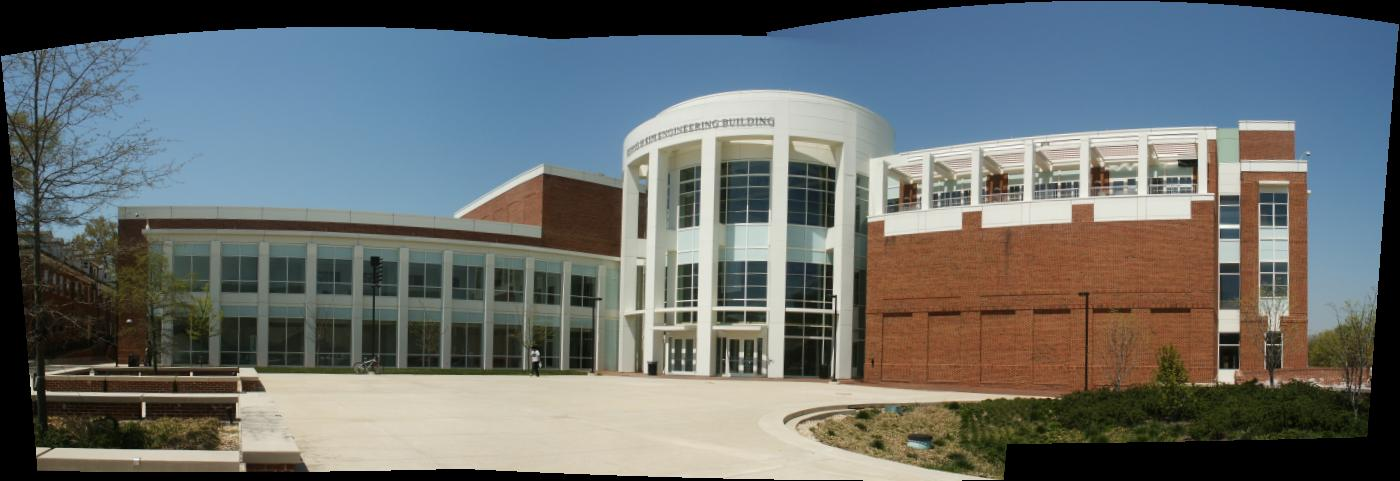
\includegraphics[width=10cm]{../../images/KIM/pano.eps}\\
        \end{center}
      \end{minipage}
    \end{tabular}
  \end{center}
\end{figure}
\end{slide}
\section[tocsection=true,slide=false]{References}

\begin{slide}{Selected References}
  \bibliographystyle{siam}
  \nobibliography{../report/SIFT}
  (1) \bibentry{dLowe04} \\ \vspace{10pt}
  (2) \bibentry{cHarris88} \\ \vspace{10pt}
  (3) \bibentry{cTomasi91} \\ \vspace{10pt}
  (4) \bibentry{mBrown03} \\ \vspace{10pt}
\end{slide}


\end{document}
